\documentclass[11pt,a4paper]{article}

% ---------- packages ----------
\usepackage[utf8]{inputenc}
\usepackage[T1]{fontenc}
\usepackage[a4paper,margin=2.4cm]{geometry}
\usepackage{graphicx}
\usepackage{booktabs}
\usepackage{tabularx}
\usepackage{array}
\usepackage{xcolor}
\usepackage{caption}
\usepackage{enumitem}
\usepackage{listings}
\usepackage{amssymb}
\usepackage[hidelinks]{hyperref}

\graphicspath{{figures/}}
\captionsetup{font=small,labelfont=bf}
\setlist{nosep,leftmargin=1.4em}

% monospace listing style for the ADTrees / topology blocks
\definecolor{codebg}{gray}{0.96}
\lstset{
  basicstyle=\ttfamily\footnotesize,
  backgroundcolor=\color{codebg},
  frame=none, breaklines=true, columns=fullflexible,
  keepspaces=true, xleftmargin=0.6em, aboveskip=0.6em, belowskip=0.6em,
}
\newcommand{\code}[1]{\texttt{\small #1}}

% ---------- title ----------
\title{\textbf{Threat Detection, Monitoring and Prevention\\in a Large-Scale Service Architecture}}
\author{Security in Large-Scale Systems --- Project 1\\Universidade de Aveiro}
\date{2026}

\begin{document}
\maketitle

\begin{abstract}
\noindent
We design and operate a service-oriented architecture (SOA) that scales horizontally and is
instrumented for both \emph{performance} and \emph{security} observability, and we exercise it
against four network threats: a distributed denial of service, an email spam campaign, a
command-and-control (C2) channel, and a man-in-the-middle interception (the last as a bonus).
For each threat we build the attack, detect it with Prometheus and/or the Wazuh SIEM, correlate
symptoms to a root cause following the FCAPS fault-management workflow, and apply an automatic or
operator action-response. The approach is \emph{measured rather than asserted}: a probe confirms
the attack surface by real request, an injected fault shows alert-cascade correlation collapsing
to its root cause, and a scalability study produces the security lesson that controls must key on
\emph{identity} rather than address. Every result is reproduced on an isolated Incus lab inside a
single VM and backed by captured evidence.
\end{abstract}

% =====================================================================
\section{Introduction}
Large-scale operators run thousands of service instances; attacks are inevitable and mostly
leave resource traces even when logs are tampered with. The problem is therefore not only
\emph{prevention} but \textbf{detection at scale} and \textbf{fast localization} of the incident
source. This project builds a representative (small but structurally faithful) system and shows,
end to end, how three required threat classes --- plus one bonus --- are detected, correlated and
mitigated. We reuse the tools from the practical guides: Incus (VIM), a Python SOA, Prometheus
(monitoring) and Wazuh (SIEM).

\noindent\textbf{Contributions.}
\begin{itemize}
  \item A horizontally-scalable SOA with hierarchical, location-aware naming that makes incident
        localization cheap.
  \item A two-plane monitoring stack: Prometheus for availability/performance, Wazuh for security
        events, both wired to the same managed system, with Alertmanager inhibition for root-cause
        correlation.
  \item Four worked threats with reproducible PoCs, detection rules, action-responses and honest
        post-mortems.
  \item A measured attack surface, a demonstrated alert-cascade correlation, and a scalability
        study whose result feeds back into the security design (per-identity rate limiting).
\end{itemize}

% =====================================================================
\section{Relevant State of the Art}
\begin{itemize}
  \item \textbf{FCAPS (ISO/IEC 7498-4)} --- the telecom management model. We focus on \emph{Fault}
        management (Detect $\rightarrow$ Isolate/Diagnose $\rightarrow$ Correlate $\rightarrow$
        Resolve/Mitigate $\rightarrow$ Post-mortem) and note that FCAPS Fault does \textbf{not}
        cover explicit security events, which is why a SIEM is added alongside.
  \item \textbf{ETSI NFV / VIM} --- virtual infrastructure managed by a VIM; here Incus plays the
        VIM role (containers as virtualized network functions).
  \item \textbf{Attack-surface \& Attack-Defense Trees} --- MITRE CAPEC domains (communications,
        software, social engineering) frame the threats; ADTrees (Kordy et al.) structure attacker
        goals versus defenses and are used per threat in \S\ref{sec:risk}.
  \item \textbf{Monitoring} --- Prometheus (pull-based time series, exporters, alerting) is the
        de-facto cloud-native standard, and its Alertmanager groups, de-duplicates and
        \emph{inhibits} alerts; Wazuh (open-source SIEM, OSSEC lineage) provides log management,
        decoders/rules, FIM and active-response. SpamAssassin (Bayesian + rule scoring) and
        Metasploit (C2/offensive tooling) are standard references for the spam and C2 threats.
\end{itemize}

% =====================================================================
\section{Service Architecture}\label{sec:arch}
\begin{figure}[htbp]
  \centering
  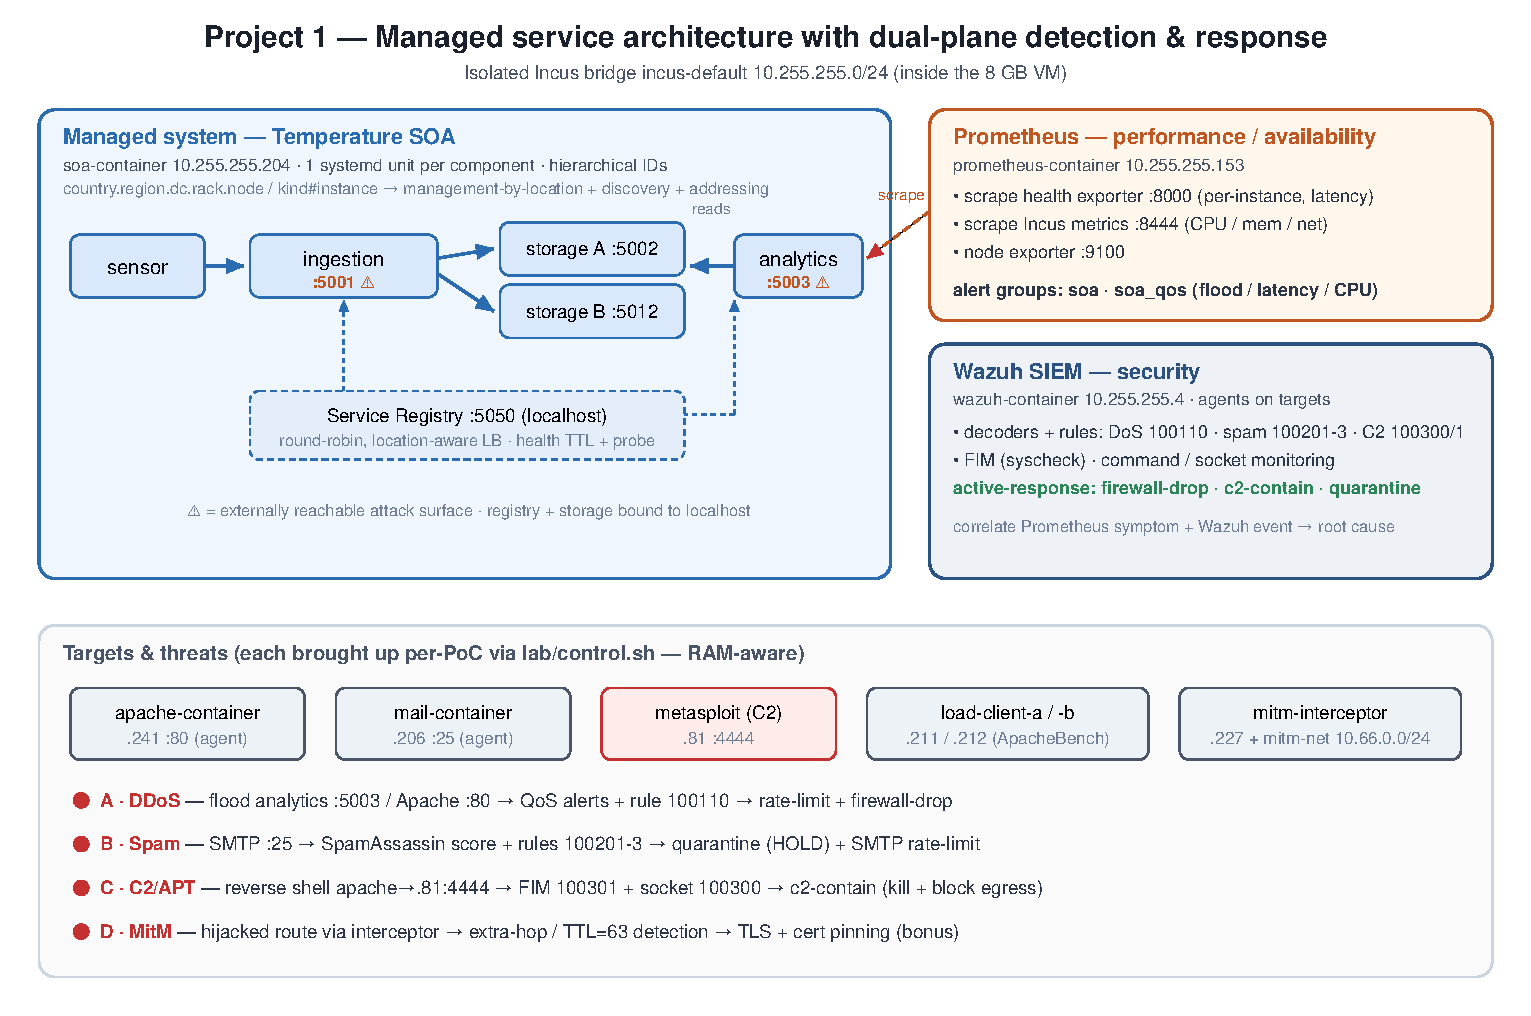
\includegraphics[width=0.84\linewidth]{architecture.pdf}
  \caption{The managed temperature SOA on the isolated Incus bridge, monitored by two planes
  (Prometheus for performance/availability, Wazuh for security), with the four threats and their
  detection/response paths. Only externally reachable services ($\triangle$) are attack surfaces;
  the registry and storage replicas are localhost-bound.}
  \label{fig:arch}
\end{figure}

The managed system is a temperature-telemetry SOA, deployed in \code{soa-container} and run as one
\code{systemd} unit per component:
\begin{lstlisting}
 sensor -> ingestion(:5001) -> storage x2 (:5002/:5012, SQLite) <- analytics(:5003)
                        \ discover/register /
                   Service Registry (:5050, round-robin LB, health TTL + active probe)
\end{lstlisting}

\paragraph{Scalability \& large-scale properties (project ``key aspects'').}
\begin{itemize}
  \item \textbf{Identification/registration} --- every instance has a hierarchical ID
        \code{country.region.datacenter.rack.node / service-kind \# instance} (e.g.
        \code{pt.aveiro.dc1.rack02.node04/storage-service\#5012}). The prefix supports
        \emph{management by location}, the kind supports \emph{discovery}, the suffix gives
        \emph{addressing}.
  \item \textbf{Physical vs logical placement} --- the location prefix encodes datacenter/rack/node;
        the registry can filter/aggregate per location
        (\code{/services?location=pt.aveiro.dc1}).
  \item \textbf{Delegation \& load balancing} --- discovery is round-robin and \emph{location-aware}
        (\code{near=} prefers same-rack/same-DC instances), so traffic and bandwidth stay local.
  \item \textbf{Fast incident localization} --- because IDs carry location, an alert naming a
        \code{service\_id} immediately tells you \emph{where} (which rack/node) to look.
\end{itemize}

\paragraph{Monitoring planes.}
\emph{Prometheus} (\code{prometheus-container}) scrapes a custom health/application exporter
(per-instance liveness, request/error/latency), the \textbf{Incus metrics endpoint} (per-container
CPU/mem/net --- more accurate than an in-container node exporter under LXC), and a node exporter;
Alertmanager collects the fired alerts. \emph{Wazuh} (\code{wazuh-container}) runs agents on the
targets and provides decoders, correlation rules, FIM and active-response. Addressing (all on the
isolated \code{incus-default} bridge \code{10.255.255.0/24}): wazuh \code{.4}, prometheus
\code{.153}, soa \code{.204}, apache \code{.241}, mail \code{.206}, C2 \code{.81}.

% =====================================================================
\section{Risk Management and Mitigation}\label{sec:risk}

\subsection{Measured attack surface}\label{sec:surface}
Rather than list the attack surface on paper, a throwaway \textbf{probe}
(\code{threats/00-attack-surface/probe.sh}) sends one real request per candidate exposure from the
realistic adversary position --- already on the service network, holding no credentials, running
\emph{inside} \code{soa-container} because the registry and storage replicas are localhost-bound and
only reachable after a foothold --- and records whether each is confirmed or blocked. It confirmed
\textbf{6 of 7} (Table~\ref{tab:surface}).

\begin{table}[htbp]
\centering\small
\caption{Measured attack surface. Each row is confirmed by a real request from a foothold.}
\label{tab:surface}
\begin{tabularx}{\linewidth}{@{}l l X l@{}}
\toprule
\textbf{Exposure} & \textbf{Probe request} & \textbf{Result} & \textbf{Status}\\
\midrule
Discovery poisoning  & \code{POST /register} decoy, then \code{/discover} & \code{/discover} returns the attacker URL & Confirmed\\
One-request DoS       & \code{DELETE /unregister} a live instance & one request evicts it (restored after) & Confirmed\\
Forged data           & \code{POST /ingest} a plausible ghost reading & accepted (shape/range \emph{is} checked, identity is not) & Confirmed\\
Topology leak         & \code{GET /services} & returns the labelled rack/node map & Confirmed\\
Open monitoring plane & unauth \code{GET} Prometheus API & metrics and alerts readable (Wazuh API auth-gated) & Confirmed\\
Plaintext transport   & \code{http} vs \code{https} to a service & plain HTTP, HTTPS refused & Confirmed\\
\bottomrule
\end{tabularx}
\end{table}

\noindent\textbf{Controls that held} (also recorded by the probe): lab isolation (no egress),
unprivileged systemd-hardened containers, and the localhost-binding of the registry and storage
replicas, which keeps them off the pre-foothold surface. Finding on forged data is more precise
than ``no validation'': ingestion \emph{does} validate shape and physical range (an out-of-range
\code{999.9} is rejected with HTTP~400) but not device identity, so a forged value within range is
stored indistinguishably from a real one --- this motivates the per-identity control in
\S\ref{sec:identity}.

\subsection{Consolidated attack--defense tree and ranked residual risk}
The per-threat ADTrees in \S\ref{sec:t1}--\S\ref{sec:t4} condense into one tree. \code{[impl]} is a
deployed control with a verifying test; \code{[gap]} is a weakness left open on purpose; \code{C} is
a counter-defense (how an attacker defeats the control above it).
\begin{lstlisting}
Goal: compromise the telemetry SOA
|- A1 Deny service (OR)                [impl] per-identity limiter + Wazuh firewall-drop
|    |- Flood the expensive endpoint    [impl] Prometheus QoS alerts + per-IP rate-limit
|    |                                   C: distributed flood keeps each IP under quota
|    \- One-request kill (/unregister)   [gap] registry write endpoints unauthenticated
|- A2 Persistent control / C2 (AND)    [impl] FIM + port-agnostic egress detection + auto-contain
|    |- Deliver + run payload            [impl] FIM on drop dirs; no toolchain in image
|    |- Reverse-shell egress             [impl] detect unexpected egress; kill + block
|    |                                   C1: HTTPS C2 on :443   C2: memory-only payload
|    \- Persistence                      [gap] autostart FIM only; no re-image
|- A3 Intercept traffic / MitM (OR)    [impl] route-hijack detection (extra hop, TTL=63)
|    \- Read/alter plaintext HTTP        [gap] no TLS between services
|                                        C: TLS + pinning/HSTS would close it (future work)
\- A4 Corrupt / forge data (OR)        [impl] shape + physical-range validation at ingestion
     |- Forge a reading                   [gap] no device authentication
     \- Poison discovery                   [gap] registry write endpoints unauthenticated
\end{lstlisting}

\noindent\textbf{Ranked residual risk} (ease of attack $\times$ impact; each is a bridge to
Project~2's attack-tolerance work):
\begin{enumerate}[label=\arabic*.]
  \item \textbf{No auth on the registry's write endpoints} --- discovery poisoning and a
        one-request DoS.
  \item \textbf{No auth on the monitoring plane} --- the Prometheus API is an open read; in a full
        deployment, Alertmanager silences would let an attacker mute their own detection.
  \item \textbf{No device authentication at ingestion} --- forged readings are accepted.
  \item \textbf{No TLS between services} --- plaintext is readable and alterable on-path.
  \item \textbf{Registry is a single in-memory point of failure} --- it also loses state on restart.
  \item \textbf{Single-node SIEM / single central Prometheus} --- availability couples to one host.
  \item \textbf{Behavioural C2 detection is evadable} --- HTTPS-on-:443 or a memory-only payload.
\end{enumerate}
The previously-ranked lack of per-client rate limiting was \emph{closed} during the DoS work and is
now an \code{[impl]} node with its own counter-defense (distributed flood) --- see
\S\ref{sec:identity}.

% ---------- threat 1 ----------
\subsection{Threat A --- Massive Denial of Service (DDoS)}\label{sec:t1}
\textbf{Description.} Availability attack: exhaust CPU/workers/connections so legitimate users are
denied service. The analytics \code{/anomalies} endpoint is expensive (reads $\le$1000 rows +
statistics per call) --- a natural pressure point.

\noindent\textbf{ADTree.}
\begin{lstlisting}
Deny analytics availability
 --> Flood expensive endpoint (/anomalies)  ..> per-IP rate limit; QoS alert
 --> Many sources at once (distributed)      ..> upstream filtering / autoscaling / reputation
 --> Exhaust connections                     ..> reverse-proxy timeouts, conn limits
\end{lstlisting}

\noindent\textbf{Exploitation.} Two lab containers (\code{load-client-a/b}) run ApacheBench against
the analytics endpoint; two simultaneous sources emulate a small botnet. Bounded and time-boxed.

\noindent\textbf{Monitoring (Prometheus, group \code{soa\_qos}).} \code{DoS\_RequestFlood}
(rate $>$10 req/s), \code{QoSDegraded\_AnalyticsLatency} (\code{/health} probe $>$0.05\,s),
\code{DoS\_TargetCPUSaturated} (CPU $>$0.8 core), all \code{for:30s}. Wazuh rule 100110 catches an
HTTP flood ($\ge$60 req/10\,s from one source) on Apache's access log.

\noindent\textbf{Action-response.} Prometheus side: per-IP rate limit (\code{remediate.sh}, iptables
hashlimit). Wazuh side: \code{firewall-drop} blocks the flooding IP.

\noindent\textbf{Post-mortem.} Baseline \code{/health} 5\,ms $\rightarrow$ attack 202\,ms; CPU
0.04 $\rightarrow$ 1.64 cores; analytics server p95 33 $\rightarrow$ 488\,ms. With the rate limit:
CPU held at 0.25 cores, \code{/health} back to 3\,ms, the legitimate client served in 17\,ms, 958
SYNs dropped (Figure~\ref{fig:dos}). \emph{Limitation:} a per-IP limit does not stop a
\emph{distributed} flood (each IP keeps its quota), and ApacheBench ``failed'' counts are
length-mismatches --- \emph{throughput alone does not prove availability loss}; latency and
saturation do.

\begin{figure}[htbp]
  \centering
  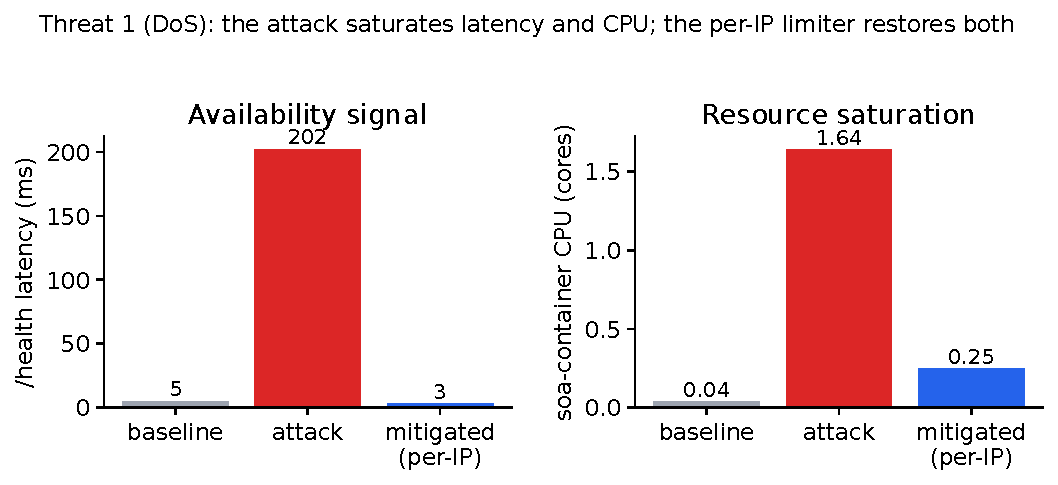
\includegraphics[width=0.92\linewidth]{fig_dos.pdf}
  \caption{Threat 1 (DoS): the attack saturates \code{/health} latency (5$\rightarrow$202\,ms) and
  CPU (0.04$\rightarrow$1.64 cores); the per-IP limiter restores both (3\,ms, 0.25 cores).}
  \label{fig:dos}
\end{figure}

% ---------- threat 2 ----------
\subsection{Threat B --- Junk Email / Spam}
\textbf{Description.} Unsolicited mail: social-engineering fraud (phishing lures) and volume
(availability/storage/cost). A multi-tenant operator must filter, quarantine and rate-limit.

\noindent\textbf{ADTree.}
\begin{lstlisting}
Deliver spam / abuse the MTA
 --> Social-engineering content   ..> SpamAssassin scoring + quarantine
 --> High volume                  ..> SMTP per-client rate limit (anvil)
 --> Reuse sending IP             ..> reputation blocklist (CDB / Bayes)
\end{lstlisting}

\noindent\textbf{Architecture \& exploitation.} \code{mail-container}: Postfix (MTA) + Dovecot +
SpamAssassin, with \code{smtpd -> content\_filter=spamassassin -> spamc -> spamd}. \code{spam.py}
sends \code{gtube} (deterministic spam), \code{social} (prince/lottery/bank phish) and
\code{volume N} (flood). A readying bug was found and fixed (spamd not running; on Ubuntu the unit
is \code{spamassassin.service}, configured via \code{/etc/default/spamassassin}).

\noindent\textbf{Monitoring \& response (Wazuh).} A PCRE2 decoder extracts the SpamAssassin score;
rules 100201 (any spam), 100202 (high-confidence $\ge$100), 100203 (campaign: $\ge$10 spam in
60\,s). Response (\code{mail\_controls.sh}): quarantine flagged mail to the HOLD queue and a Postfix
anvil per-client rate limit.

\noindent\textbf{Post-mortem.} GTUBE scored 1003/5.0; 16 spam sent with quarantine on
$\rightarrow$ 16 held, 0 delivered; rules 100201/2/3 all fired; rate limit: 15 messages
$\rightarrow$ 10 accepted, 5 rejected. \emph{Limitation:} GTUBE guarantees a verdict; real spam
needs trained Bayes and risks false positives --- hence quarantine (reversible) over hard reject.

% ---------- threat 3 ----------
\subsection{Threat C --- Command-and-Control / Botnet (APT)}
\textbf{Description.} A C2 server remotely controls compromised hosts (a botnet). A reverse shell
gives interactive control through outbound-only firewalls. Detecting and cutting the channel limits
an APT.

\noindent\textbf{ADTree.}
\begin{lstlisting}
Establish & keep C2 on a host
 --> Deliver + run payload        ..> FIM on drop dirs; execution monitoring
 --> Reverse shell egress to C2   ..> detect unexpected egress; kill + block
 --> Persistence (cron/systemd)   ..> FIM on autostart; re-image
\end{lstlisting}

\noindent\textbf{Exploitation (safety-gated).} All traffic stays on \code{10.255.255.0/24};
\code{payload.sh} refuses any non-lab \code{LHOST}. A Kali \code{metasploit-container} C2 runs an
\code{msfvenom} x64 \code{reverse\_tcp} payload and a \code{multi/handler}; the payload executes on
\code{apache-container} $\rightarrow$ a meterpreter session over the bridge.

\noindent\textbf{Monitoring (Wazuh, two angles).} Rule 100301 (FIM realtime on the drop dir) catches
the payload; rule 100300 (command monitoring every 15\,s) catches the live C2 connection and is
\textbf{port-agnostic}: any \emph{outbound} ESTABLISHED connection a web server initiates to a lab
host (excluding DNS and the Wazuh manager) is the reverse shell, so 4444, 443, 8080 or a random port
are flagged alike.

\noindent\textbf{Action-response (\code{c2-contain.sh}, automatic, persistent).} Finds the web
server's outbound shell, kills the owning process, and DROPs egress to that peer in a dedicated
\code{C2-CONTAIN} chain --- again port-agnostic.

\noindent\textbf{Post-mortem.} Session opened (\code{.81:4444 -> .241}); FIM and C2 alerts both
fired; containment killed the process and blocked egress; re-run payload $\rightarrow$ 0
connections. \emph{Limitations:} detection latency $\approx$ one 15\,s poll (an EDR with kernel
socket hooks would be immediate); the ``no outbound from a web server'' heuristic needs a per-role
allow-list; containment cuts the channel but not persistence.

% ---------- threat 4 ----------
\subsection{Threat D --- Man-in-the-Middle / Route hijacking (bonus)}\label{sec:t4}
\textbf{Description.} An on-path attacker intercepts/alters traffic, relevant to the ``route and
signals hijacking'' syllabus item.

\noindent\textbf{ADTree.}
\begin{lstlisting}
Intercept client<->service traffic
 --> Become the route (gateway/hop)   ..> routing hardening; detect extra hop/TTL
 --> Read/alter HTTP                   ..> TLS everywhere
 --> Present a bogus certificate       ..> cert pinning / HSTS
\end{lstlisting}

\noindent\textbf{Exploitation --- implemented and demonstrated.} An isolated second subnet
(\code{mitm-net}) places \code{mitm-client} so its only route to Apache is through
\code{mitm-interceptor} (a hijacked route; no ARP spoofing). The interceptor forwards
(\code{ip\_forward} + MASQUERADE) and captures the full plaintext (\code{GET / HTTP/1.1},
\code{Server: Apache/2.4.52}, the page body) --- confidentiality loss. A second \code{active} mode
proves \textbf{integrity} loss: an \code{iptables} REDIRECT sends the forwarded \code{:80} into a
pure-stdlib transparent proxy (\code{active\_mitm.py}, recovering the target via
\code{SO\_ORIGINAL\_DST}) that rewrites the response; the client received an injected banner and a
\code{(TAMPERED)} title the server never served.

\noindent\textbf{Detection \& response.} Client-side \code{traceroute} shows an extra hop
(\code{10.66.0.2}) and \code{ttl=63} instead of 64 --- the route-hijack signal. TLS is what closes
the threat: it makes the body ciphertext the proxy cannot rewrite, and pinning/HSTS makes an active
attacker's substitute certificate fail; routing hardening (\code{accept\_redirects=0}) complements
it. (mitmproxy is unpackaged on Debian trixie, so both read and active modes use the standard
library only.)

% =====================================================================
\section{Evaluation and Scalability}\label{sec:eval}

\subsection{Effectiveness}
Each required threat is detected \emph{and} mitigated, verified with evidence: DoS QoS alerts +
rate-limit (CPU 1.64 $\rightarrow$ 0.25 cores under attack); spam fully quarantined and rate-limited;
C2 channel detected and auto-severed in $\le$15\,s; the MitM route-hijack detected by hop/TTL.
Correlating Prometheus (performance) with Wazuh (security) is what localizes root cause.

\subsection{Root-cause correlation, demonstrated}\label{sec:corr}
A failure in a service-oriented architecture produces a \emph{cascade} of alerts: the one broken
dependency plus every downstream symptom. We added Alertmanager inhibition rules
(\code{monitoring/alertmanager.yml}) to the Prometheus plane and injected a single fault, a
\textbf{storage-tier outage} (both SQLite replicas stopped). It fired \textbf{4 alerts}: 2 root
causes (\code{ServiceDown} on each storage replica) and 2 downstream symptoms
(\code{HighErrorRatio} on the ingestion and analytics services, which depend on storage).
Inhibition suppresses a symptom while its cause is firing, so the operator is shown
\textbf{only the 2 causes} (Figure~\ref{fig:corr}). A dual experiment confirmed the mechanism:
stopping the \emph{registry} makes the pipeline go \emph{silent} (clients can no longer discover
each other), so only \code{RegistryDown} fires --- a clean single cause with no cascade. The
cascade's size scales with the number of instances, so correlation matters more as the system
grows.

\begin{figure}[htbp]
  \centering
  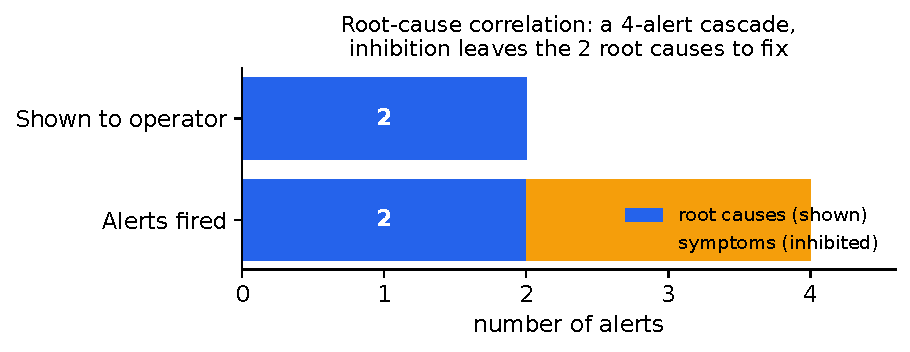
\includegraphics[width=0.82\linewidth]{fig_correlation.pdf}
  \caption{A 4-alert cascade from one injected fault; Alertmanager inhibition leaves only the 2 root
  causes the operator must act on.}
  \label{fig:corr}
\end{figure}

\subsection{Scalability}\label{sec:scale}
One node was made to host $N$ sensors ($N$ distinct hierarchical identities behind one source IP)
and the ingestion pipeline measured at $N=10/50/100$ (Table~\ref{tab:scale},
Figure~\ref{fig:scale}).

\begin{table}[htbp]
\centering\small
\caption{Pipeline scalability: one node hosting $N$ sensors.}
\label{tab:scale}
\begin{tabular}{@{}rrrrr@{}}
\toprule
\textbf{Sensors} & \textbf{Throughput (req/s)} & \textbf{p50 (ms)} & \textbf{p95 (ms)} & \textbf{soa CPU (cores)}\\
\midrule
10  & 88 & 23  & 651  & 0.99\\
50  & 93 & 73  & 2823 & 1.06\\
100 & \textbf{12} & 3002 & 3005 & 0.59\\
\bottomrule
\end{tabular}
\end{table}

Throughput saturates near \textbf{90 req/s at roughly one core} (the Flask/GIL path plus a
synchronous storage POST per request), and at 100 concurrent closed-loop clients it
\textbf{collapses to 12 req/s} with latencies pinned at the 3\,s client timeout: the connection
burst overruns the HTTP server's accept queue, threads stall in timeout (so CPU \emph{drops}), and
the pipeline stops making progress. Raising server concurrency (worker pool, async I/O, or a reverse
proxy) is the documented next step.

\begin{figure}[htbp]
  \centering
  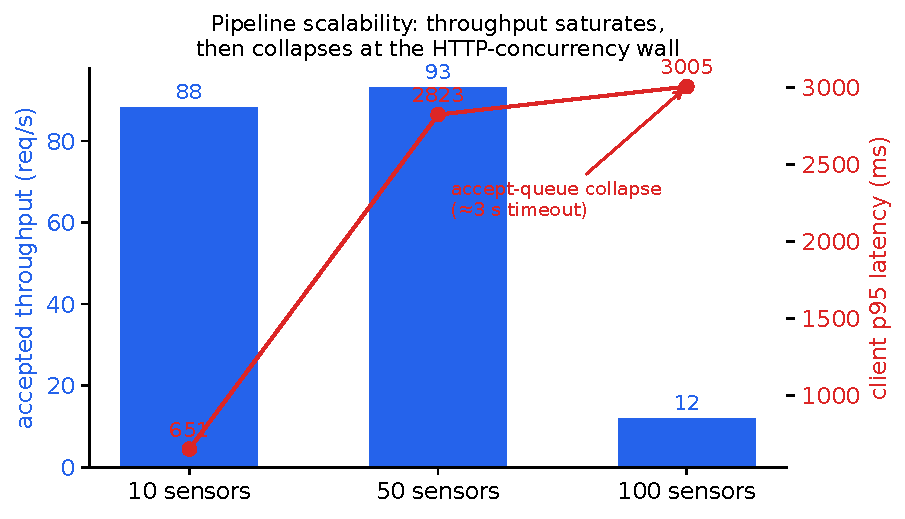
\includegraphics[width=0.78\linewidth]{fig_scalability.pdf}
  \caption{Throughput saturates then collapses at the HTTP-concurrency wall at 100 sensors.}
  \label{fig:scale}
\end{figure}

\subsection{The security finding: per-IP controls misfire at scale}\label{sec:identity}
The scale test exposes a security lesson. The DoS defense (\code{remediate.sh}) is an \code{iptables}
hashlimit keyed on \textbf{source IP}. But one node hosts many sensors, so its \emph{aggregate}
connection rate trips a per-IP limit even though every individual sensor is well-behaved --- the
control then denies the service it protects. Measured with 50 legitimate sensors from one IP
(Table~\ref{tab:identity}, Figure~\ref{fig:identity}):

\begin{table}[htbp]
\centering\small
\caption{Keying the limiter on identity instead of address.}
\label{tab:identity}
\begin{tabularx}{\linewidth}{@{}l c c X@{}}
\toprule
\textbf{Control} & \textbf{Legit served} & \textbf{Throughput} & \textbf{Flood reusing one identity}\\
\midrule
per-IP (iptables hashlimit) & 49.9\,\% (685 SYNs dropped) & 11 req/s & n/a\\
per-identity (token bucket on \code{device\_id}) & \textbf{94.5\,\%} & 70 req/s & \textbf{shed: 682 $\times$ HTTP 429}\\
\bottomrule
\end{tabularx}
\end{table}

Keying the limiter on the sensor's \textbf{hierarchical identity} instead of its address
(\code{architecture/ratelimit.py}, env-gated hook in \code{ingestion\_service.py}, default off) gives
each sensor its own token bucket (5 req/s, burst 10): the legitimate node is served, and a flood that
reuses a single identity is still shed. This closes the project's own stated future-work item and
ties the scalability result straight back into the security design.

\begin{figure}[htbp]
  \centering
  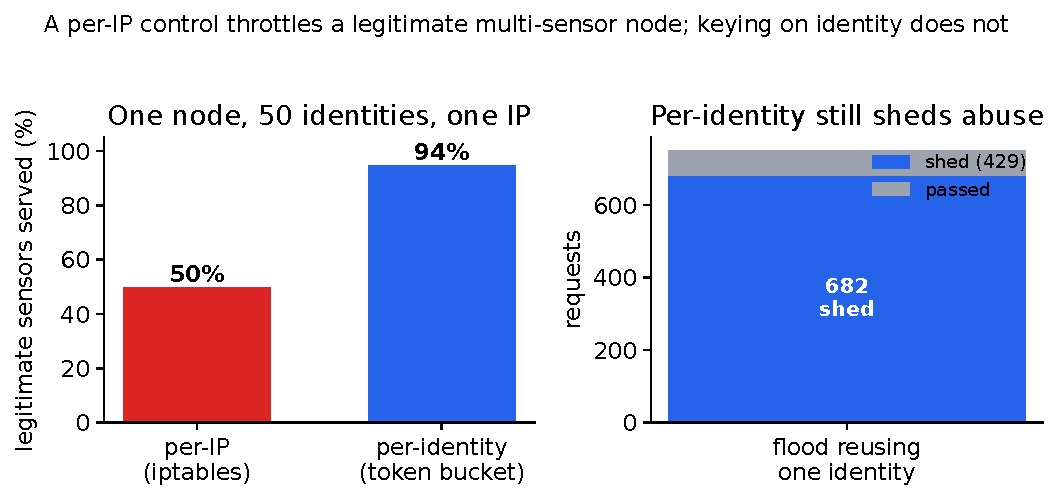
\includegraphics[width=0.9\linewidth]{fig_identity_vs_ip.pdf}
  \caption{A per-IP control throttles a legitimate 50-identity node (49.9\,\% served); keying on
  identity serves it (94.5\,\%) and still sheds a single-identity flood.}
  \label{fig:identity}
\end{figure}

\noindent\textbf{Honest residue.} The per-identity run still shows $\sim$5\,\% legit failures and a
p95 at the timeout, because the HTTP-concurrency wall from Figure~\ref{fig:scale} is a \emph{different}
bottleneck: the limiter fixes the false positive, not the server's accept-queue ceiling. The two
controls protect different properties --- integrity of the data store (the limiter) versus
availability under a connection burst (server concurrency) --- and neither substitutes for the other.

\subsection{Other scaling limits}
On an 8\,GB single VM the whole stack cannot run at once (Wazuh indexer alone $\approx$2.3\,GB); PoCs
are sequenced with \code{lab/control.sh}. At true scale the indexer and Prometheus would be their own
clusters --- a known, documented constraint, not a design flaw.

% =====================================================================
\section{Conclusions}
A structurally-faithful large-scale SOA was built, instrumented on two planes and defended against
four threats with reproducible PoCs, SIEM integration and action-responses, all following the FCAPS
fault workflow. The main findings concern method as much as mechanism: the attack surface was
\emph{measured} rather than assumed (\S\ref{sec:surface}); an alert cascade was correlated down to its
root cause by Alertmanager inhibition (\S\ref{sec:corr}); and a scalability study produced the lesson
that a security control keyed on source address will, at scale, mistake legitimate aggregation for an
attack --- so controls must key on \emph{identity} (\S\ref{sec:identity}). Every mitigation has a cost
and a gap, and documenting the gap (distributed DoS, spam false positives, C2 persistence, single-node
SIEM) is itself a result. \textbf{Future work:} mTLS + authenticated registry writes, a reputation
service shared across threats, flow-based C2 detection, raising HTTP-server concurrency, and
clustering the SIEM/monitoring for real scale --- bridging toward Project~2's attack-tolerance
mechanisms.

\paragraph{Reproducibility.}
\code{lab/genesis.sh} rebuilds the core; \code{siem/install\_siem.sh} installs all
detection/response; \code{monitoring/install-alertmanager.sh} adds the correlation plane;
\code{threats/*/README.md} run each PoC; and every figure and headline number traces to a capture
script and a raw evidence file (Table~\ref{tab:evidence}).

\begin{table}[htbp]
\centering\footnotesize
\caption{Evidence map: each report item traces to a script and a raw file.}
\label{tab:evidence}
\setlength{\tabcolsep}{4pt}
\begin{tabular}{@{}>{\raggedright\arraybackslash}p{4.2cm} l l@{}}
\toprule
\textbf{Report item} & \textbf{Produced by} & \textbf{Raw evidence}\\
\midrule
Measured attack surface (Table~\ref{tab:surface}) & \code{threats/00-attack-surface/probe.sh} & \code{evidence/attack-surface-*.txt}\\
Correlation (Fig.~\ref{fig:corr}) & \code{tools/correlation-demo.sh} & \code{evidence/correlation-*.txt}\\
Scalability (Table~\ref{tab:scale}, Fig.~\ref{fig:scale}) & \code{tools/scalability-sweep.sh} & \code{evidence/scalability-*.csv}\\
Identity vs IP (Table~\ref{tab:identity}, Fig.~\ref{fig:identity}) & \code{tools/identity-vs-ip-demo.sh} & \code{evidence/identity-vs-ip-*.txt}\\
DoS before/after (Fig.~\ref{fig:dos}) & \code{threats/01-ddos/run.sh} & \code{threats/01-ddos/evidence/}\\
Threats B/C/D PoCs & \code{threats/0\{2,3,4\}-*/} & \code{threats/0\{2,3,4\}-*/evidence/}\\
SIEM rules + active response & \code{siem/install\_siem.sh} & Wazuh manager alerts\\
\bottomrule
\end{tabular}
\end{table}

\section*{Declaration on the Use of AI}
\addcontentsline{toc}{section}{Declaration on the Use of AI}
An AI coding assistant was used throughout this project as a productivity tool, under the
author's direction and review. Specifically, it supported: \emph{implementing the services}
(the SOA registry, ingestion, storage, analytics and sensor components and their
instrumentation); \emph{generating the tests and load/attack drivers} used to exercise and
measure the system; \emph{implementing the threat proof-of-concepts} (DDoS, spam, C2 and the
on-path MitM) together with their detections and active responses; \emph{running the
experiments and collecting the results} that appear in this report (the attack-surface probe,
the correlation demonstration, and the scalability and identity-vs-IP studies); and
\emph{drafting the report} itself. All generated artefacts were read, tested on the live lab,
corrected and validated by the author, who takes full responsibility for the design decisions,
the correctness of the measurements and the claims made herein.

\end{document}
